\documentclass[12pt, aspectratio=169]{beamer}

\usepackage{color}
\usepackage[utf8]{inputenc}
\usepackage{graphicx}
\usepackage{tikz}
\usepackage[T1]{fontenc}
\usepackage{caption}
\usepackage{wrapfig}
\usepackage{xurl}
\usepackage{pgfplots}
\usepackage{minipage-marginpar}
\usepackage{wrapfig}
\usepackage{subfig}


\captionsetup[figure]{labelformat=empty}
\setbeamertemplate{section in toc}[square]

\usetheme{Singapore}
\usecolortheme{default}
\usefonttheme{structurebold}
\setbeamerfont{text}{size=\large}
\setbeamercovered{dynamic}
\setbeamertemplate{bibliography item}{\insertbiblabel}
\pgfplotsset{compat=1.16}

\definecolor{ao}{rgb}{0.0, 0.0, 0.7}

%\setbeamertemplate{footline}[frame number]
\setbeamertemplate{footline}[text line]{%
  \parbox{\linewidth}{\vspace*{-8pt}\color{ao}\insertshorttitle\hspace{10px}\insertshortauthor\hfill\insertpagenumber}}

\title{Test mittels Heuristischer Evaluation}
\author[Y. Höll, F. Jäpel, C. Pooch]{Yannik Höll \& Franz Jäpel \& Christoph Pooch}
\date{April 26, 2022}
% \logo{
\includegraphics[keepaspectratio=True, width=30px]{./image/logo.png}}



\beamertemplatenavigationsymbolsempty 

\begin{document}
\begin{frame}[noframenumbering, plain]
	\titlepage
\end{frame}

\begin{frame}
	\frametitle{Einteilung}
	\tableofcontents
\end{frame}

\section{System Usability Scale}
\begin{frame}
\begin{center}
	\begin{table}	
	\begin{tabular}{|c|c|c|c|c|c|c|c|c|c|c|}
	\hline
	\textbf{Frage}& \textbf{1}& \textbf{2} & \textbf{3} & \textbf{4} & \textbf{5} & \textbf{6} & \textbf{7} & \textbf{8} & \textbf{9} & \textbf{10} \\ \hline
	\textbf{Tester 1}&1	&2 &4 &1 &3	&3 &4 &2 &3	&1 \\ \hline
	\textbf{Tester 2}&1	&1 &4 &2 &5 &2 &4 &1 &3 &1 \\ \hline
	\textbf{Tester 3}&1	&3 &3 &2 &2 &3 &2 &2 &3 &3 \\ \hline
	\textbf{Tester 4}&2	&1 &4 &2 &4 &1 &4 &1 &4 &1 \\ \hline
	\textbf{Tester 5}&2	&3 &4 &2 &4 &4 &3 &4 &3 &1 \\ \hline
	\textbf{Tester 6}&2	&2 &4 &4 &3 &1 &5 &3 &3	&3 \\ \hline
	\textbf{Durchschn.}&1,50 &2,00 &3,83 &2,17 &3,50 &2,33 &3,67 &2,17 &3,17 &1,67 \\ \hline
		\end{tabular}
	\caption{Auswertung SUS Fragebogen}
	\end{table}
\end{center}
\end{frame}

\begin{frame}
	\begin{figure}	
		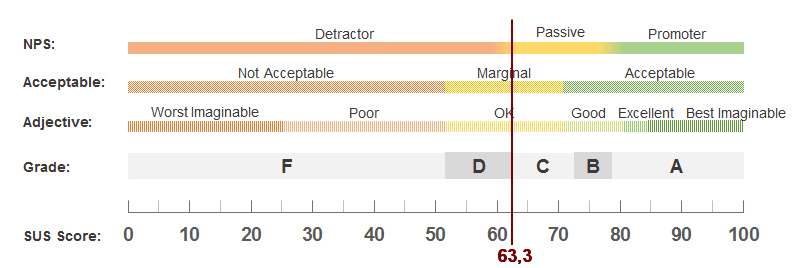
\includegraphics[width=1\textwidth]{image/sus-scale-nocorrect.png}
		\caption{Auswertung SUS Fragebogen mittels Skalierung}
	\end{figure}
\end{frame}

\begin{frame}
	\begin{tikzpicture}
	\begin{axis}[
        ylabel={Punktzahl},
		xlabel={Frage},
		title=Durschnittliche Punktzahl pro Frage,
		ybar,
		nodes near coords, bar width=0.2cm,
		symbolic x coords={1, 2, 3, 4, 5, 6, 7, 8, 9, 10},
        width=\textwidth,
        height=0.9\textheight
	]
	\addplot coordinates{(1, 1.5)(2, 2)(3, 3.83)(4, 2.17)(5, 3.5)(6, 2.33)(7, 3.67)(8, 2.17)(9, 3.17)(10, 1.67)};
	\end{axis}
\end{tikzpicture}

\end{frame}

\begin{frame}
	\begin{figure}
		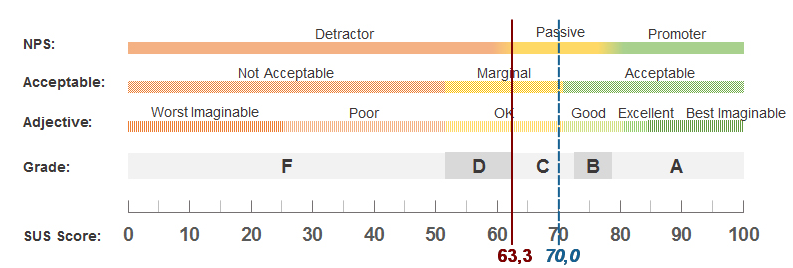
\includegraphics[width=1\textwidth]{image/sus-scale-correct.png}
		\caption{Korrigierte Auswertung SUS Fragebogen mittels Skalierung}
	\end{figure}
\end{frame}

\section{Aufgabenbewertung}
\begin{frame}
	\hspace*{-20px}
	\begin{tikzpicture}
	\begin{axis}[
		xlabel={Aufgabe},
		ylabel={Zeit in s},
		title=Zeit pro Tester und Aufgabe,
		ybar,
		bar width=0.2cm,
		symbolic x coords={S1, S2.1, S2.2, S3.1, S3.2, S3.3},
		xtick={S1, S2.1, S2.2, S3.1, S3.2, S3.3},
		width=0.89\textwidth,
		height=0.9\textheight,
		legend style={
			at={(1.15,0.0)},
			anchor=south,
			column sep=1ex
		}
	]
	\addplot[style={lime,fill=lime}] coordinates {(S1, 10)(S2.1, 70)(S2.2, 0)(S3.1, 5)(S3.2, 11)(S3.3, 7)};
	\addplot[style={green,fill=green}] coordinates {(S1, 20)(S2.1, 20)(S2.2, 0)(S3.1, 0)(S3.2, 1)(S3.3, 0)};
	\addplot[style={blue,fill=blue}] coordinates {(S1, 0)(S2.1, 0)(S2.2, 0)(S3.1, 0)(S3.2, 0)(S3.3, 0)};
	\addplot[style={red,fill=red}] coordinates {(S1, 0)(S2.1, 0)(S2.2, 0)(S3.1, 0)(S3.2, 0)(S3.3, 0)};
	\addplot[style={purple,fill=purple}] coordinates {(S1, 30)(S2.1, 30)(S2.2, 30)(S3.1, 60)(S3.2, 60)(S3.3, 240)};
	\addplot[style={violet,fill=violet}] coordinates {(S1, 3)(S2.1, 30)(S2.2, 25)(S3.1, 15)(S3.2, 30)(S3.3, 30)};
	\legend{Hönig, Bär, Sukhankova, Schanck, Naumann, Leyer}
	\end{axis}
\end{tikzpicture}

% \addplot[style={green,fill=green}] coordinates {(S1, 10)(S2.1, 70)(S2.2, 0)(S3.1, 5)(S3.2, 11)(S3.3, 7)(L1, 7)(L2.1, 292)(L2.2, 0)(L2.3, 0)(L2.4, 0)(L2.5, 0)(L2.6, 0)(L2.7, 37)(L3.1, 0)(L3.2, 0)(L3.3, 0)(L3.4, 0)(L3.5, 0)}; %Hönig
% \addplot[style={green,fill=green}] coordinates {(S1, 10)(S2.1, 70)(S2.2, 0)(S3.1, 5)(S3.2, 11)(S3.3, 7)(L1, 7)(L2.1, 292)(L2.2, 0)(L2.3, 0)(L2.4, 0)(L2.5, 0)(L2.6, 0)(L2.7, 37)(L3.1, 0)(L3.2, 0)(L3.3, 0)(L3.4, 0)(L3.5, 0)}; %Hönig
% \addplot[style={green,fill=green}] coordinates {(S1, 10)(S2.1, 70)(S2.2, 0)(S3.1, 5)(S3.2, 11)(S3.3, 7)(L1, 7)(L2.1, 292)(L2.2, 0)(L2.3, 0)(L2.4, 0)(L2.5, 0)(L2.6, 0)(L2.7, 37)(L3.1, 0)(L3.2, 0)(L3.3, 0)(L3.4, 0)(L3.5, 0)}; %Hönig
% \addplot[style={green,fill=green}] coordinates {(S1, 10)(S2.1, 70)(S2.2, 0)(S3.1, 5)(S3.2, 11)(S3.3, 7)(L1, 7)(L2.1, 292)(L2.2, 0)(L2.3, 0)(L2.4, 0)(L2.5, 0)(L2.6, 0)(L2.7, 37)(L3.1, 0)(L3.2, 0)(L3.3, 0)(L3.4, 0)(L3.5, 0)}; %Hönig
% \addplot[style={green,fill=green}] coordinates {(S1, 10)(S2.1, 70)(S2.2, 0)(S3.1, 5)(S3.2, 11)(S3.3, 7)(L1, 7)(L2.1, 292)(L2.2, 0)(L2.3, 0)(L2.4, 0)(L2.5, 0)(L2.6, 0)(L2.7, 37)(L3.1, 0)(L3.2, 0)(L3.3, 0)(L3.4, 0)(L3.5, 0)}; %Hönig
% \addplot[style={green,fill=green}] coordinates {(S1, 10)(S2.1, 70)(S2.2, 0)(S3.1, 5)(S3.2, 11)(S3.3, 7)(L1, 7)(L2.1, 292)(L2.2, 0)(L2.3, 0)(L2.4, 0)(L2.5, 0)(L2.6, 0)(L2.7, 37)(L3.1, 0)(L3.2, 0)(L3.3, 0)(L3.4, 0)(L3.5, 0)}; %Hönig
% symbolic x coords={S1, S2.1, S2.2, S3.1, S3.2, S3.3, L1, L2.1, L2.2, L2.3, L2.4, L2.5, L2.6, L2.7, L3.1, L3.2, L3.3, L3.4, L3.5},
\end{frame}

\begin{frame}
	\hspace*{-20px}
	\begin{tikzpicture}
	\begin{axis}[
        xlabel={Aufgabe},
		ylabel={Zeit in s},
		title=Zeit pro Tester und Aufgabe,
		ybar,
		bar width=0.2cm,
		symbolic x coords={L1, L2.1, L2.2, L2.3, L2.4, L2.5},
		xtick={L1, L2.1, L2.2, L2.3, L2.4, L2.5},
		width=0.895\textwidth,
		height=0.9\textheight,
		legend style={
			at={(1.15,0.0)},
			anchor=south,
			column sep=1ex
		}
	]
	\addplot[style={lime,fill=lime}] coordinates {(L1, 7)(L2.1, 292)(L2.2, 0)(L2.3, 0)(L2.4, 0)(L2.5, 0)};
	\addplot[style={green,fill=green}] coordinates {(L1, 20)(L2.1, 120)(L2.2, 120)(L2.3, 240)(L2.4, 20)(L2.5, 0)};
	\addplot[style={blue,fill=blue}] coordinates {(L1, 0)(L2.1, 0)(L2.2, 0)(L2.3, 0)(L2.4, 0)(L2.5, 0)};
	\addplot[style={red,fill=red}] coordinates {(L1, 0)(L2.1, 0)(L2.2, 0)(L2.3, 0)(L2.4, 0)(L2.5, 0)};
	\addplot[style={purple,fill=purple}] coordinates {(L1, 30)(L2.1, 300)(L2.2, 300)(L2.3, 30)(L2.4, 30)(L2.5, 0)};
	\addplot[style={violet,fill=violet}] coordinates {(L1, 30)(L2.1, 50)(L2.2, 45)(L2.3, 120)(L2.4, 40)(L2.5, 30)};
	\legend{Hönig, Bär, Sukhankova, Schanck, Naumann, Leyer}
	\end{axis}
\end{tikzpicture}
\end{frame}

\begin{frame}
	\hspace*{-20px}
	\begin{tikzpicture}
	\begin{axis}[
        xlabel={Aufgabe},
		ylabel={Zeit in s},
		title=Zeit pro Tester und Aufgabe,
		ybar,
		bar width=0.15cm,
		symbolic x coords={L2.6, L2.7, L3.1, L3.2, L3.3, L3.4, L3.5},
		xtick={L2.6, L2.7, L3.1, L3.2, L3.3, L3.4, L3.5},
		width=0.89\textwidth,
		height=0.9\textheight,
		legend style={
			at={(1.15, 0.0)},
			anchor=south,
			column sep=1ex
		}
	]
	\addplot[style={lime,fill=lime}] coordinates {(L2.6,0)(L2.7,37)(L3.1,0)(L3.2,0)(L3.3,0)(L3.4,0)(L3.5,0)};
	\addplot[style={green,fill=green}] coordinates {(L2.6,20)(L2.7,3)(L3.1,5)(L3.2,5)(L3.3,20)(L3.4,20)(L3.5,0)};
	\addplot[style={blue,fill=blue}] coordinates {(L2.6,0)(L2.7,0)(L3.1,0)(L3.2,0)(L3.3,0)(L3.4,0)(L3.5,0)};
	\addplot[style={red,fill=red}] coordinates {(L2.6,0)(L2.7,0)(L3.1,0)(L3.2,0)(L3.3,0)(L3.4,0)(L3.5,0)};
	\addplot[style={purple,fill=purple}] coordinates {(L2.6,120)(L2.7,30)(L3.1,30)(L3.2,30)(L3.3,30)(L3.4,30)(L3.5,120)};
	\addplot[style={violet,fill=violet}] coordinates {(L2.6,60)(L2.7,60)(L3.1,60)(L3.2,60)(L3.3,60)(L3.4,60)(L3.5,60)};
	\legend{Hönig, Bär, Sukhankova, Schanck, Naumann, Leyer}
	\end{axis}
\end{tikzpicture}
\end{frame}

\section{Heuristische Evaluation}

\begin{frame}
	\centering
	\begin{tabular}{|l|c|}
		\hline
		\textbf{Heuristik} & \textbf{Nummer} \\ \hline
		Determinismus& 1\\ \hline
		Sprache& 2\\ \hline
		Limitierung& 3\\ \hline
		Nutzerangepasstheit& 4\\ \hline
		Einheitlichkeit& 5\\ \hline
		Bugs& 6\\ \hline
		Anpassbarkeit& 7\\ \hline
		Nutzerunterstützung& 8\\ \hline
		Rückgängigmachen von Aktionen& 9\\ \hline
		Rückmeldung& 10\\ \hline
		Fehler vermeiden& 11\\ \hline
		Selbsterklärendes Design& 12\\ \hline
		Erwartungsgemäße Funktionalität& 13\\ \hline
		Barrierefreiheit& 14\\ \hline
		
	\end{tabular}
\end{frame}

\begin{frame}
	\hspace*{-20px}
	\begin{tikzpicture}
	\begin{axis}[
        ylabel={Verstöße},
		xlabel={Heuristik},
		title=Verstöße pro Heuristik,
		ybar,
		nodes near coords, bar width=0.2cm,
		symbolic x coords={1, 2, 3, 4, 5, 6, 7, 8, 9, 10, 11, 12, 13, 14},
        xtick={1, 2, 3, 4, 5, 6, 7, 8, 9, 10, 11, 12, 13, 14},
        width=\textwidth,
        height=0.9\textheight
	]
	\addplot coordinates{(1, 0)(2, 0)(3, 0)(4, 0)(5, 0)(6, 0)(7, 0)(8, 0)(9, 0)(10, 0)(11, 0)(12, 0)(13, 0)(14, 0)};
	\end{axis}
\end{tikzpicture}

\end{frame}

\begin{frame}
	\begin{figure}
		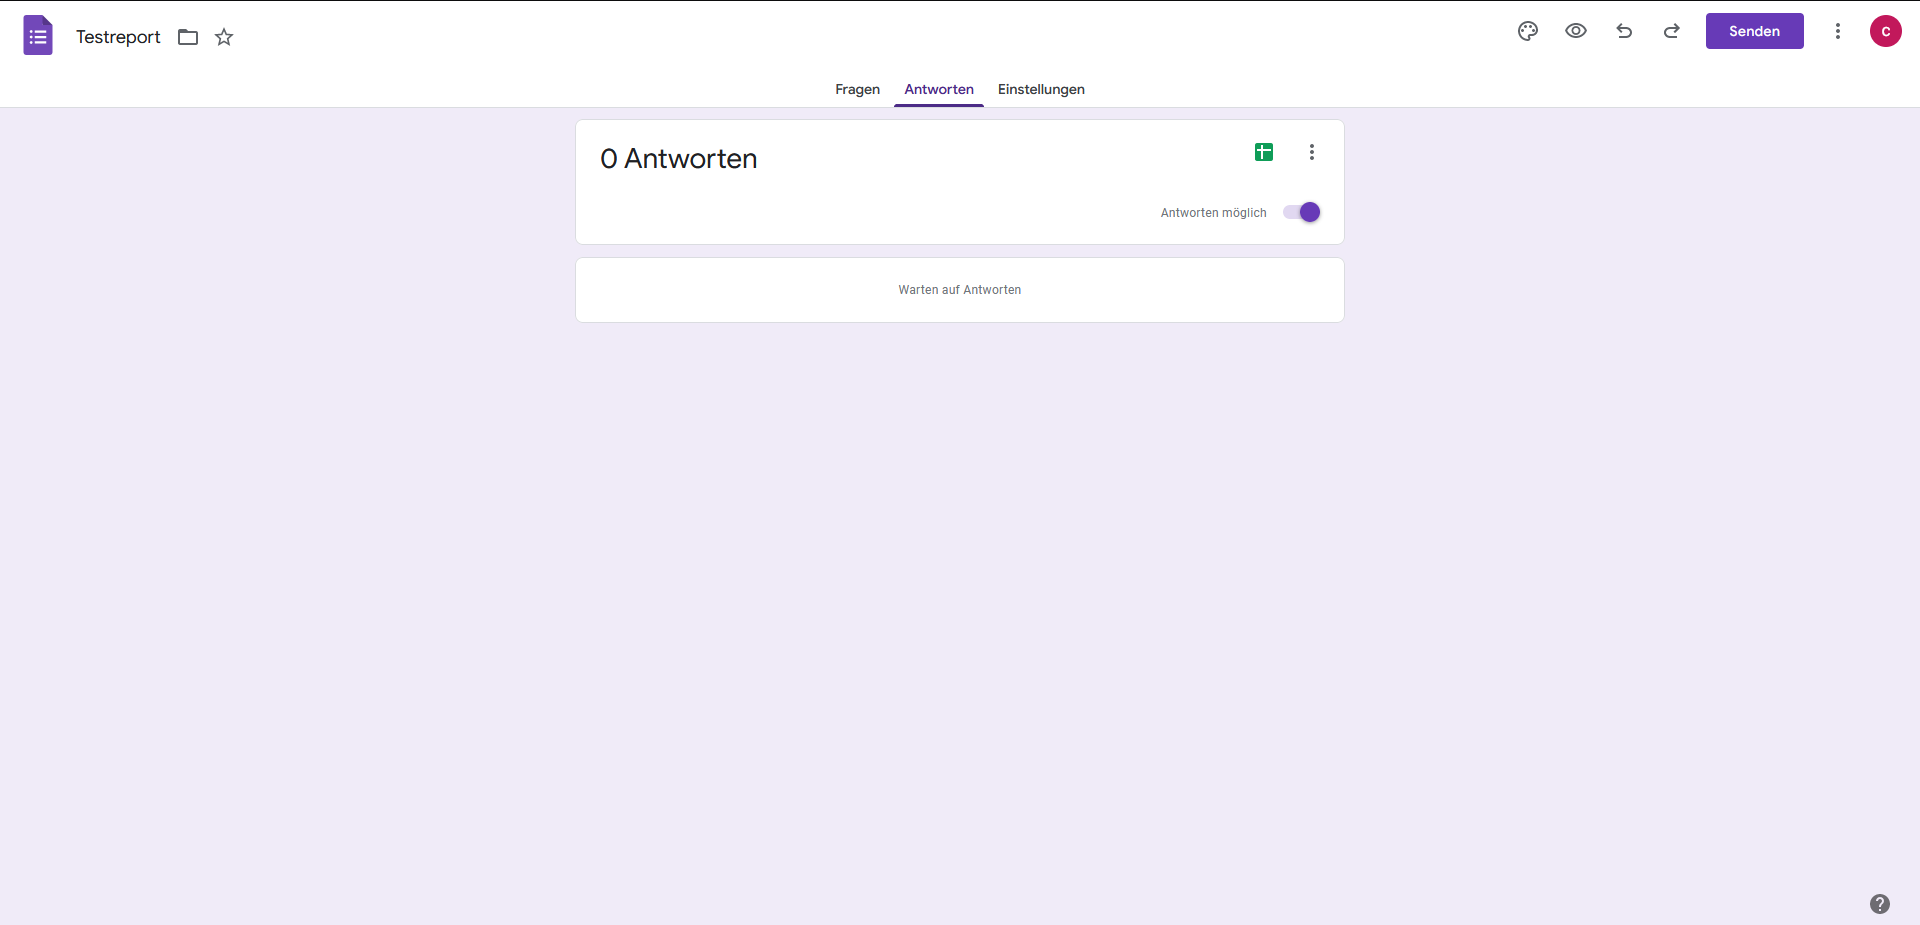
\includegraphics[height=0.6\textheight]{image/misere.png}
		\caption{Screenshot der Misere}
	\end{figure}
	\begin{enumerate}
		\item Formular Heuristiken: \url{https://forms.gle/nhwj1Xj4SPZw4Jjj6}
		\item Formular Aufgaben: \url{https://forms.gle/YQhYtWiWFfxNEUsP6}
	\end{enumerate}
\end{frame}

\begin{frame}
\begin{figure}
	\begin{minipage}[b]{0.45\linewidth}
		\centering
		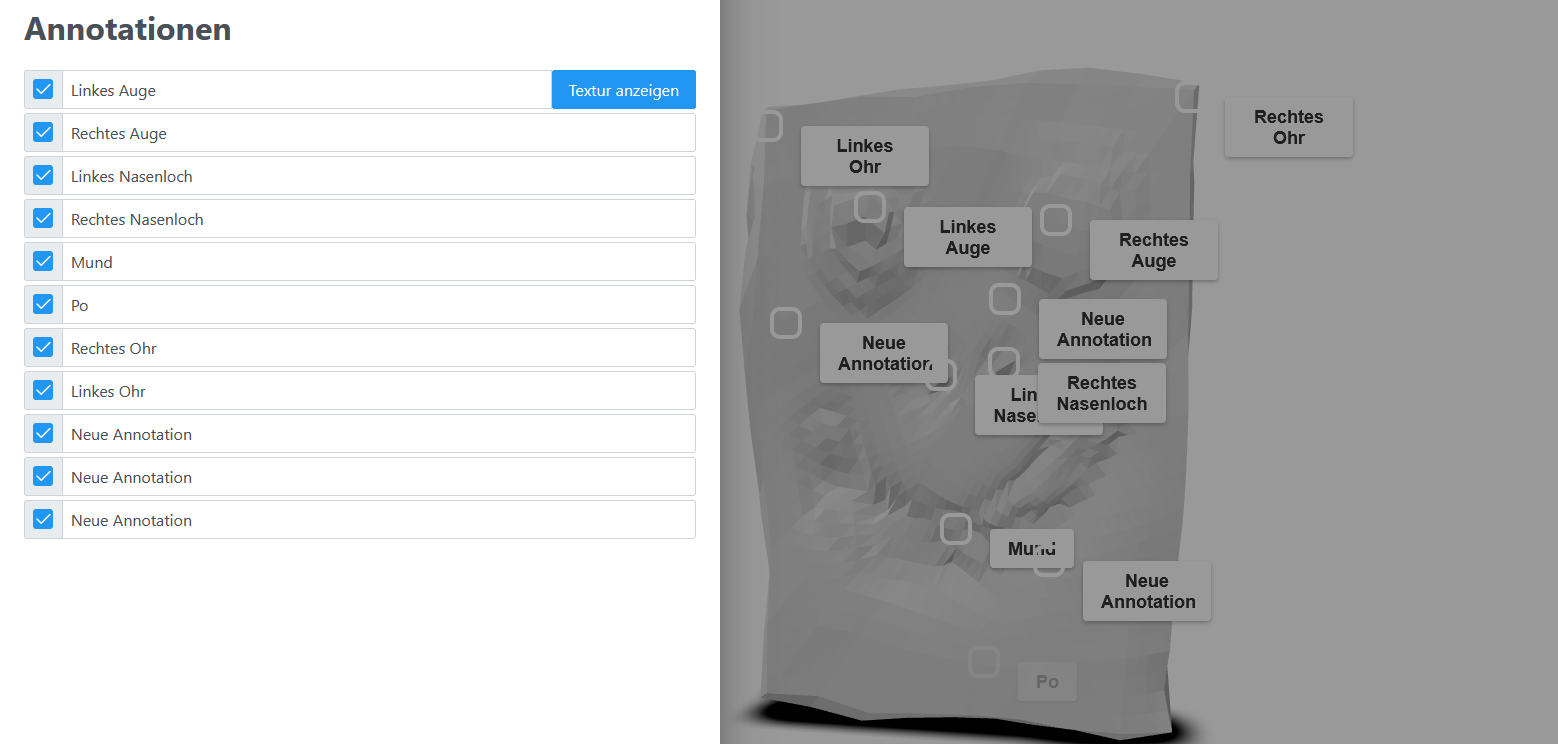
\includegraphics[width=\textwidth]{image/Heur2.png}
	\end{minipage}
	\hspace{0.5cm}
	\begin{minipage}[b]{0.45\linewidth}
		\centering
		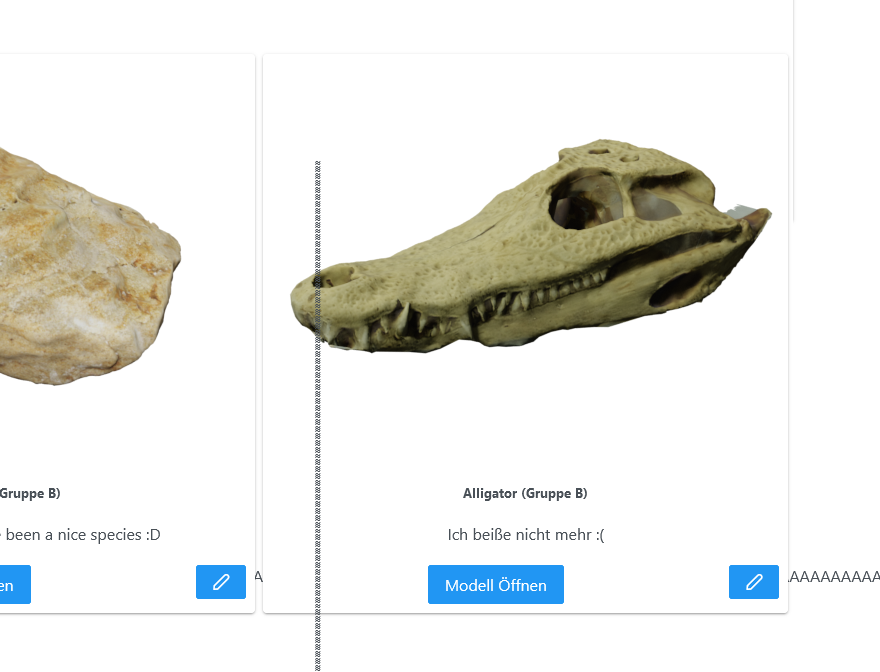
\includegraphics[width=\textwidth]{image/Heur1.png}
	\end{minipage}
	\caption{100\% der Teilnehmenden einer Heuristischen Evaluation haben hier keinen Verstoß gegen Heuristiken feststellen können!
	\ \\ Das Ergebnis war absolut genderneutral. Allerdings gab es diverse Teilnehmende nicht.\tiny{[1]}}
\end{figure}

\end{frame}

\section{Quellen}
\begin{frame}
	\centering
	\begin{figure}
		
\includegraphics[trim={0 20cm 0 15cm},clip,height=0.8\textheight]{image/geile_quelle.jpeg}
		\caption{Quelle 1 (Institut für Diskrete Mathematik und Algebra, unbekannter Autor)}
	\end{figure}
\end{frame}

\end{document}